\section{Vizualizare cheltuieli}\label{spec:receipts}

Ecranul de vizualizare a cheltuielilor (prezentat în figura \ref{fig:receipts}) este punctul de intrare în aplicație. Utilizatorul își poate vedea cheltuielile organizate pe monede, luni și categorii. În a doua jumătate a ecranului este afișată lista tuturor cheltuielilor din selecția curentă. Prin selectarea uneia, se deschide ecranul de vizualizare a unui bon fiscal (figura \ref{fig:receipt})

\begin{figure}[!ht]
  \centering
  \begin{subfigure}{0.49\textwidth}
    \centering
    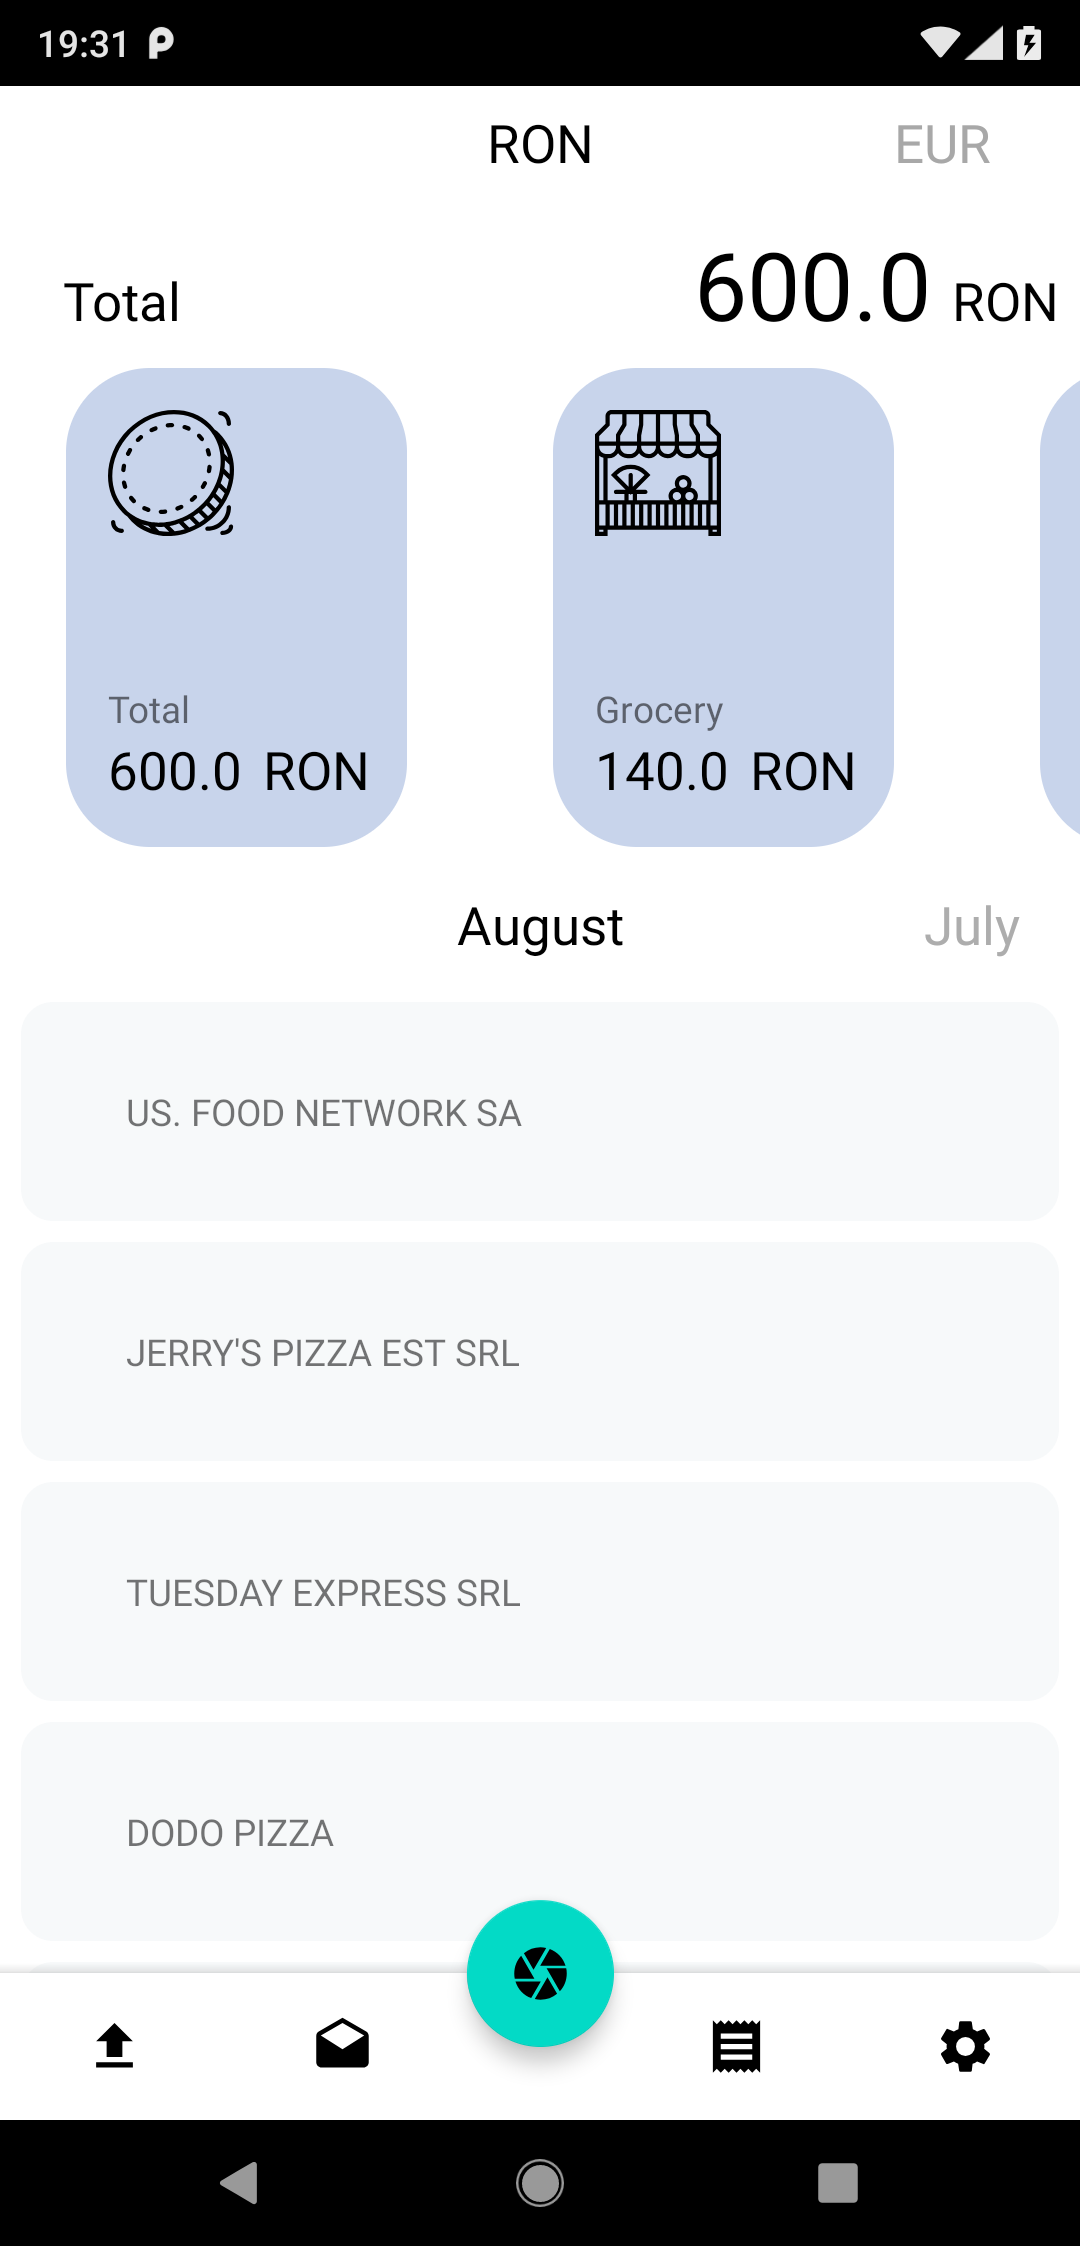
\includegraphics[width=\screenwidth]{ReceiptsScreen.png}
    \caption{Ecranul de vizualizare a cheltuielilor}
    \label{fig:receipts}
  \end{subfigure}
  \begin{subfigure}{0.49\textwidth}
    \centering
    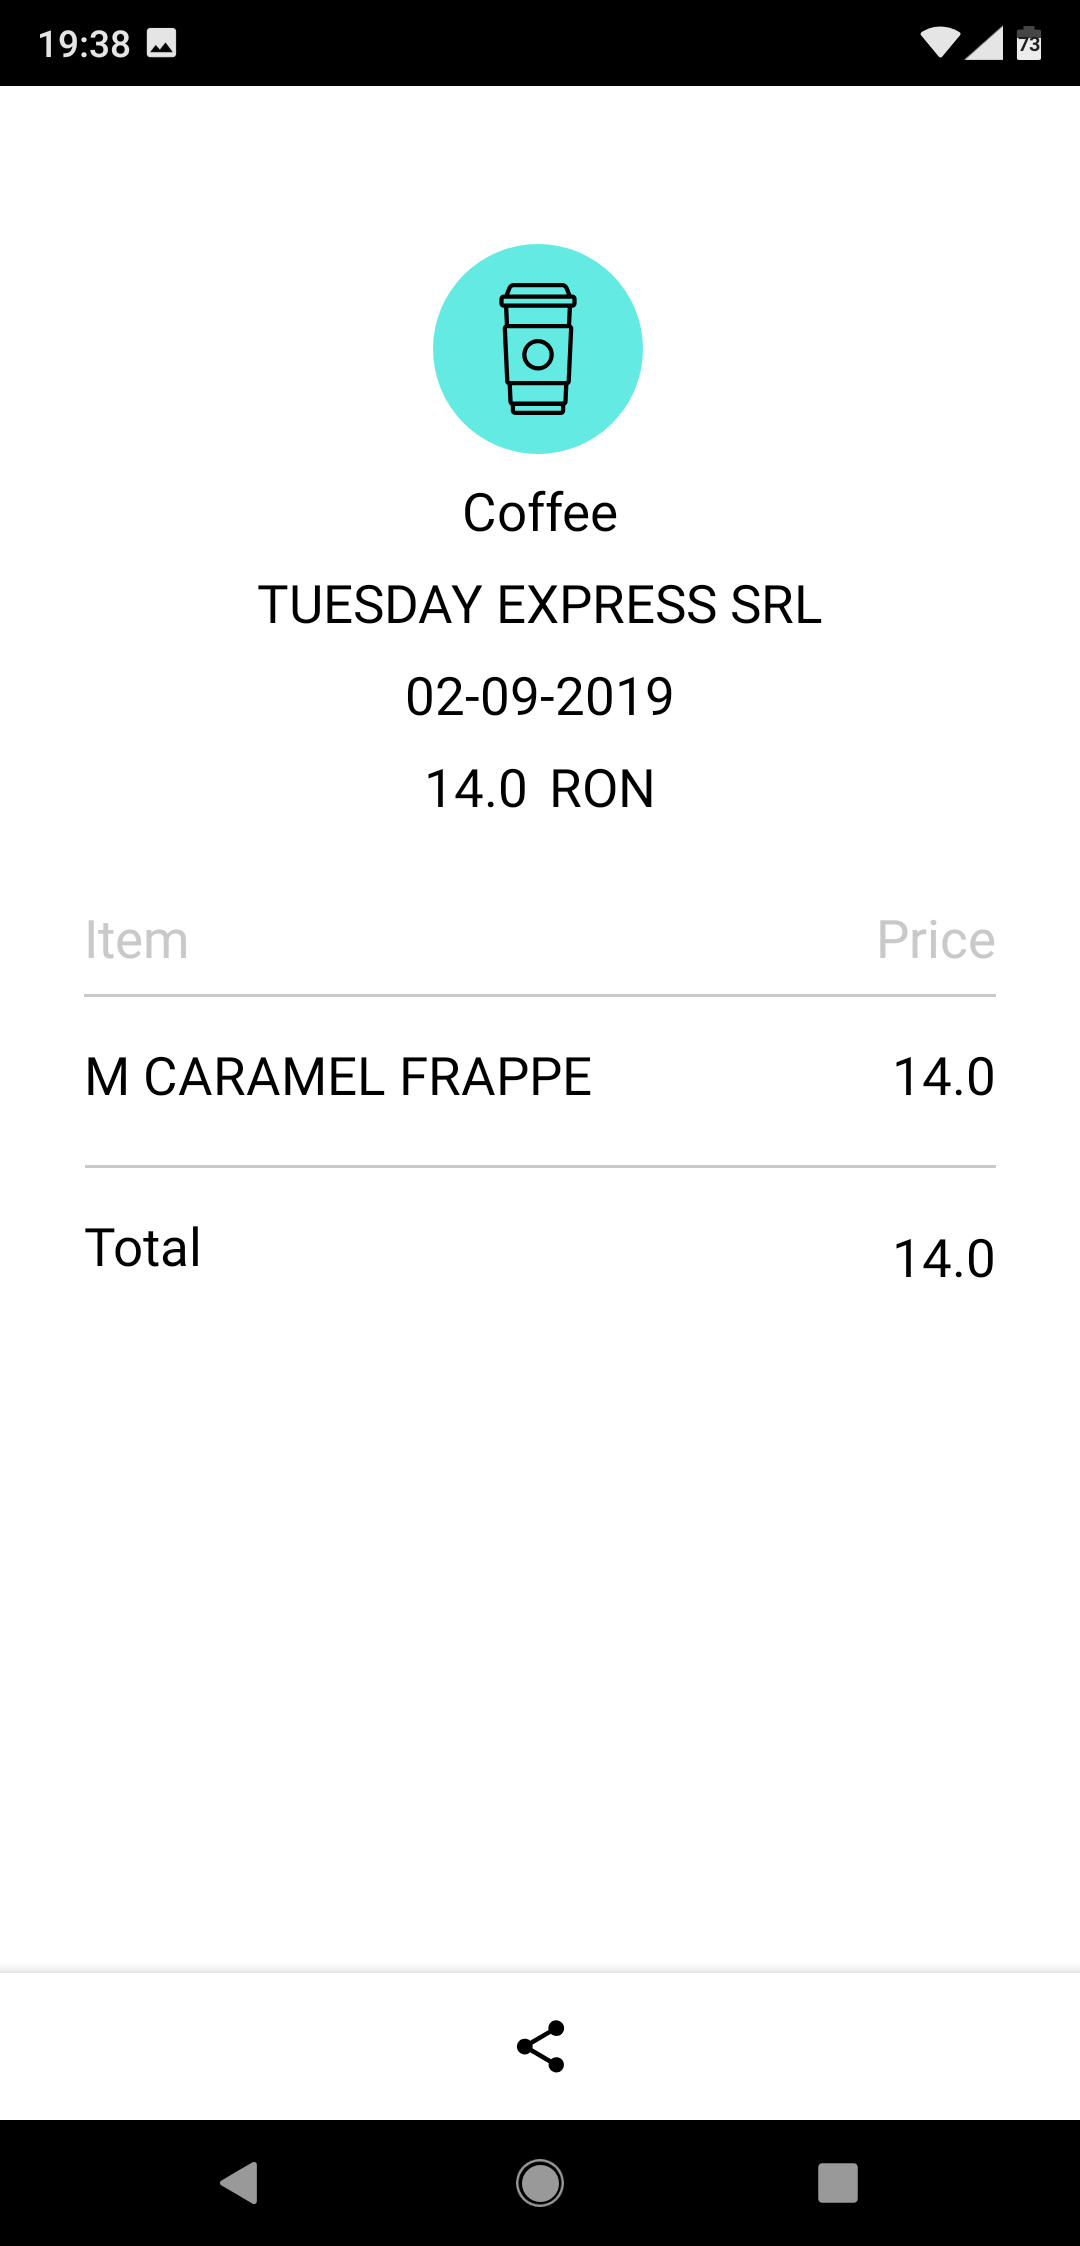
\includegraphics[width=\screenwidth]{ReceiptScreen.png}
    \caption{Ecranul de vizualizare a unui bon}
    \label{fig:receipt}
  \end{subfigure}
  \caption{Ecranele de gestionare a cheltuielilor}
  \label{fig:manageReceipts}
\end{figure}

Din ecranul de vizualizare a unui bon, utilizatorul poate trimite acel bon printr-o aplicație externă, cum ar fi clientul de \emph{e-mail} sau o aplicație de mesagerie. Motivația acestei funcționalități sunt cazurile în care cheltuielile sunt împărțite între mai multe persoane sau decontate și trebuie atașate prin \emph{e-mail}. Opțiunile de trimitere externă sunt: \emph{doar text}, \emph{doar imagine}, \emph{imagine și text}. Figura \ref{fig:sharingFlow} ilustrează procesul de distribuire externă.

\begin{figure}[!ht]
  \centering
  \begin{subfigure}{0.49\textwidth}
    \centering
    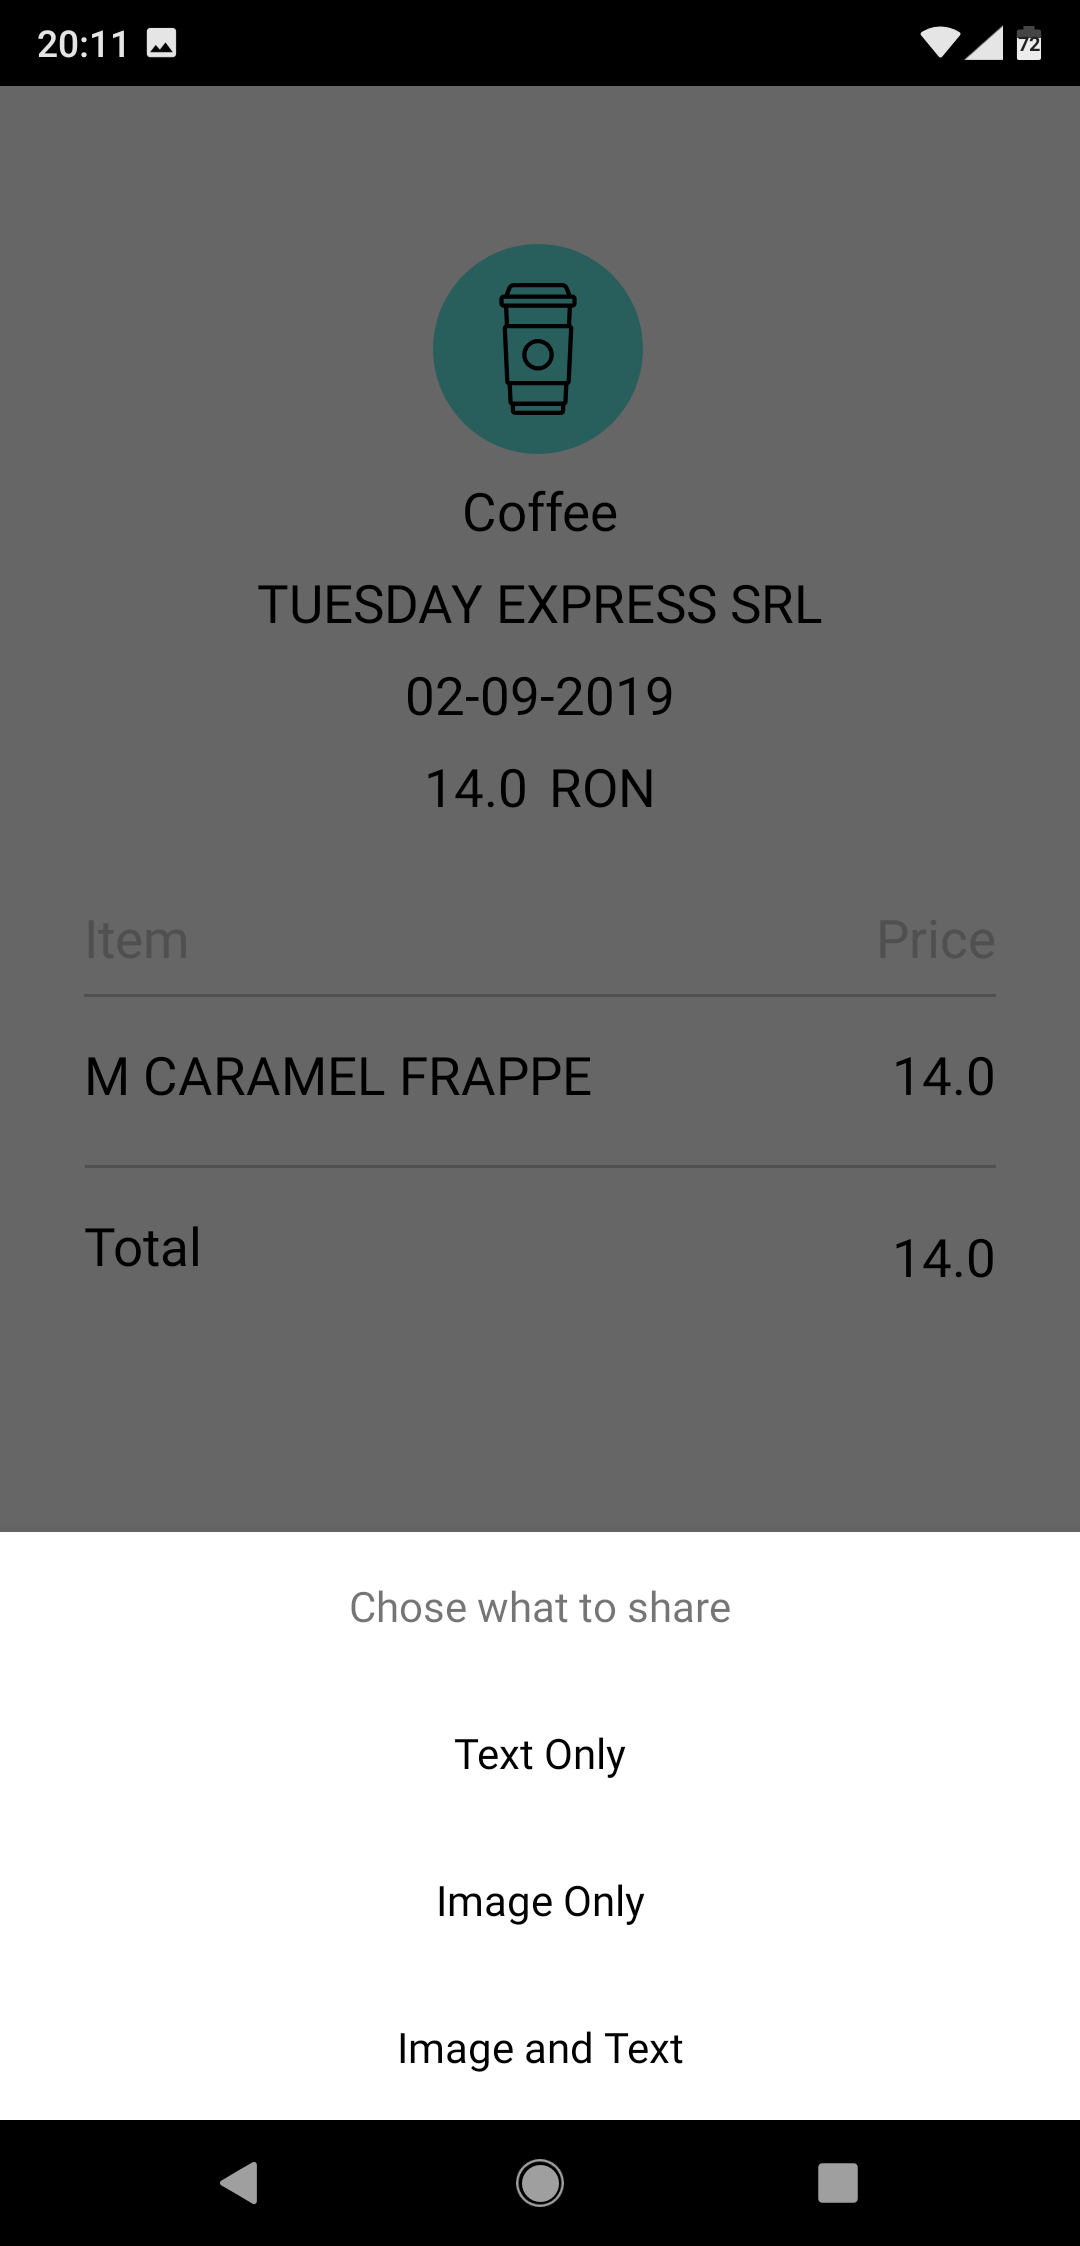
\includegraphics[width=\screenwidth]{ShareOptionsScreen.png}
    \caption{Opțiunile de trimitere externă}
    \label{fig:sharingOptions}
  \end{subfigure}
  \begin{subfigure}{0.49\textwidth}
    \centering
    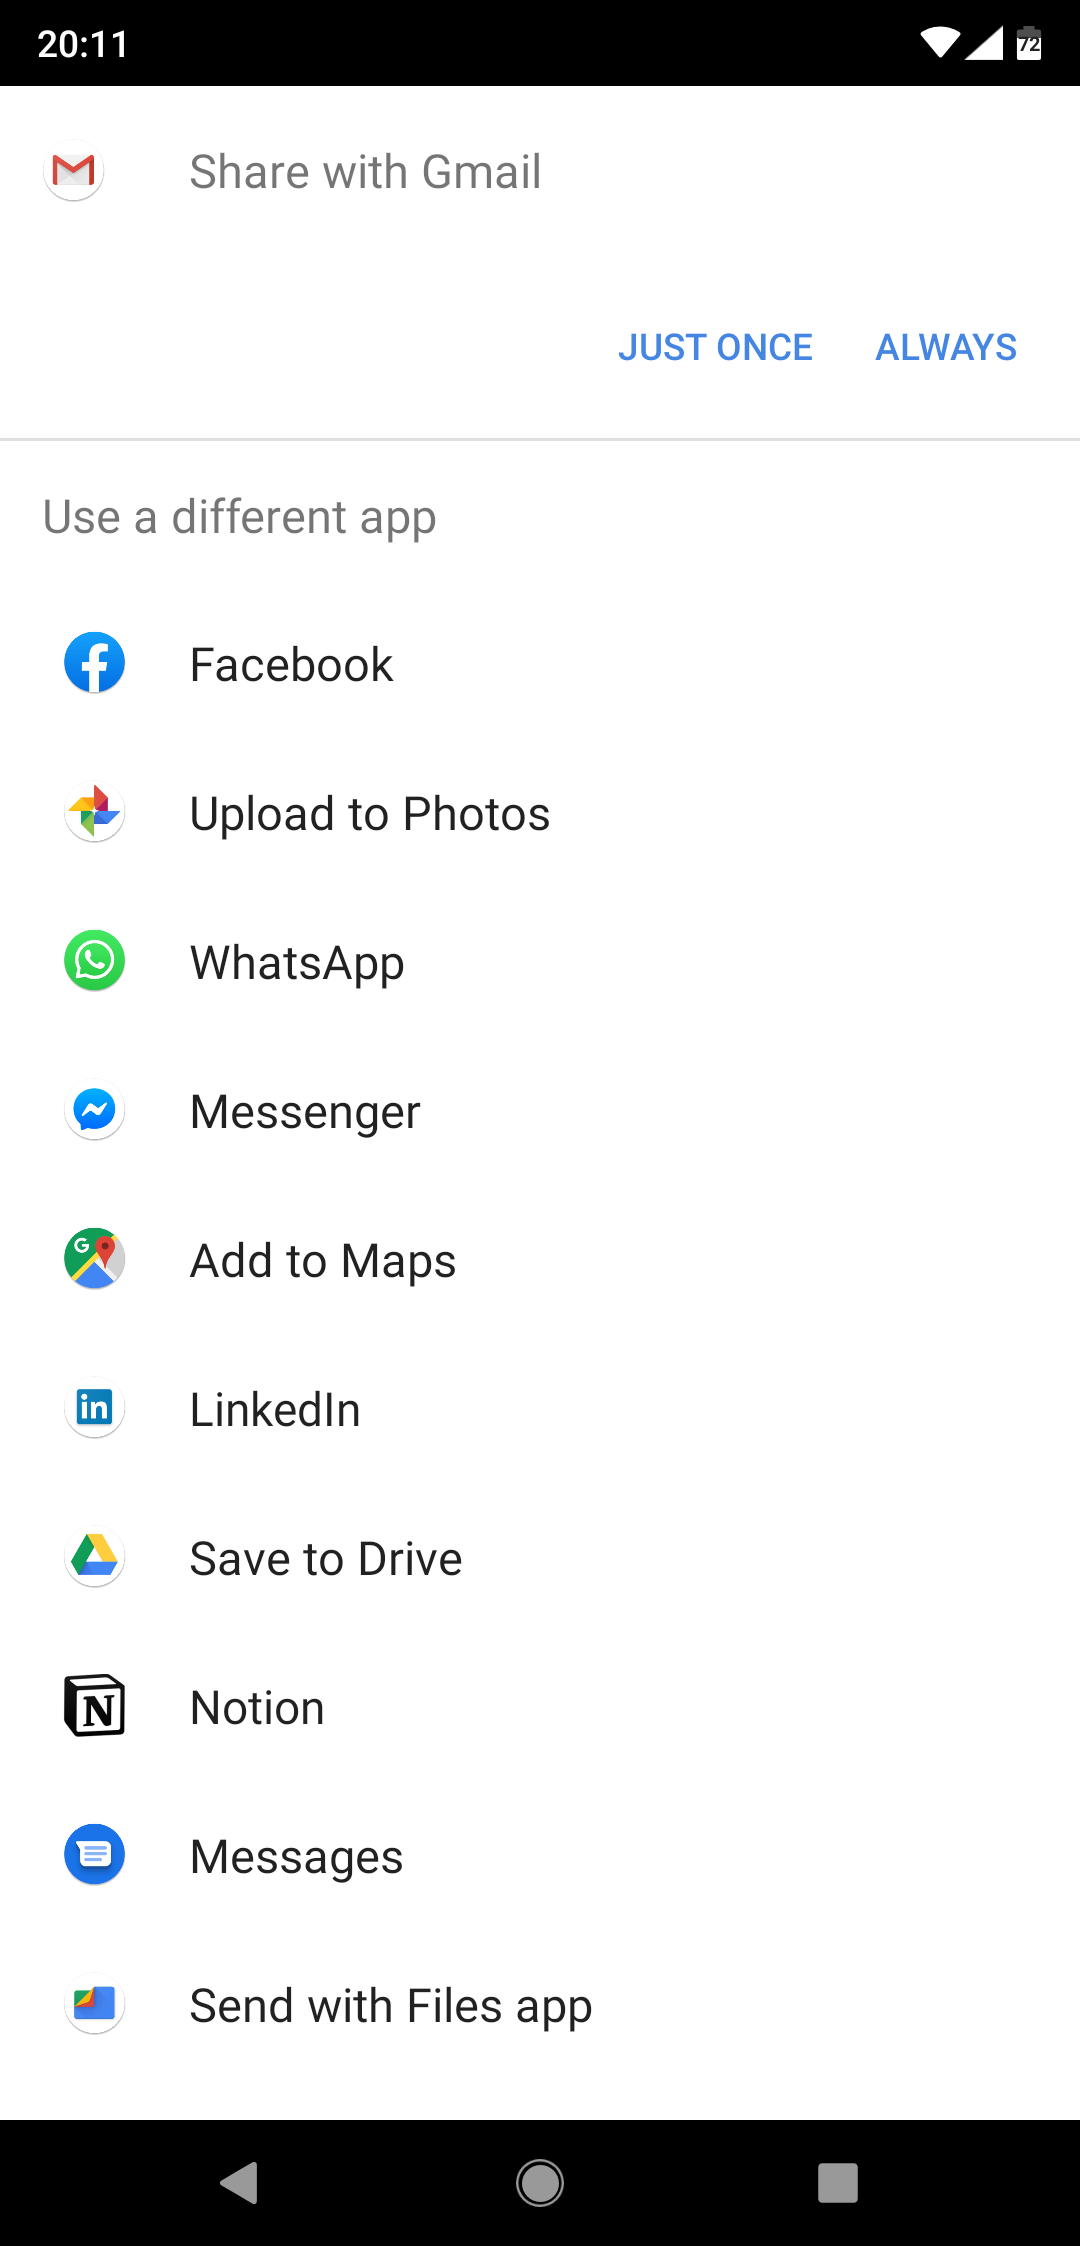
\includegraphics[width=\screenwidth]{ExternalAppsScreen.png}
    \caption{Ecranul de vizualizare a unui bon}
    \label{fig:externalApps}
  \end{subfigure}
  \caption{Aplicațiile externe prin care poate fi trimis un bon}
  \label{fig:sharingFlow}
\end{figure}

\begin{itemize}
  \item \textbf{Scop}: Vizualizarea datelor în legătură cu cheltuielile; Trimiterea informațiilor aferente unei tranzacții pe canale externe;
  \item \textbf{Condiții de succes}: Afișarea cu succes a datelor; Trimiterea cu succes către aplicații externe;
  \item \textbf{Condiții de eșec}: Neafișarea datelor când acestea există; Eșecul în a face legătura cu alte aplicații pentru a trimite un bon;
\end{itemize}

\subsection*{Mențiuni}\label{spec:updateWhenFetch}

\begin{itemize}
  \item Datele sunt afișate organizate pe monedă, lună și categorie;
  \item La nivelul afișării pe categorii, există și o opțiune de a afișa toate tranzacțiile, indiferent de categorie;
  \item Datele despre o tranzacție sunt afișate într-un ecran separat;
\end{itemize}

\section*{Scenariu principal}
\begin{enumerate}
  \item Utilizatorul deschide aplicația;
  \item Sunt interogate toate monedele și lunile disponibile și afișate datele pentru luna curentă și ultima monedă utilizată;
  \item Utilizatorul accesează o tranzacție din lista returnată;
  \item Utilizatorul distribuie această tranzacție;
\end{enumerate}

\section*{Extensii}
\begin{itemize}
  \item Utilizatorul selectează o nouă monedă, categorie sau lună, iar datele sunt actualizate;
\end{itemize}